\section{System Design}\label{sec:system-design}
This section describes how the system works without going into the implementation details.
Painting the whole system as a black-box implementation, the interface is known, but the underlying implementation is not.

\subsection{Design Goals}\label{subsec:design-goals}
The primary objective of the system is to provide a flexible environment for full-stack development.
The design emphasizes simplicity and ease of integration, allowing the components extended easily.

The key design goals are:
\begin{itemize}
    \item Simplicity - The system interface is simple and similar and the implementation of programming patterns is consistent.
    \item Modularity - The system is divided into components.
    \item Extensibility - New functionality can be added to existing components.
    \item Automation - Repetitive development tasks should be automated with AI if possible.
    \item Transparency - The system should expose clear interface for each component.
\end{itemize}

These goals reflect the prototype nature of the system, which aims to explore automation of common full-stack development tasks.

\subsection{System Overview}\label{subsec:system-overview}
The system is designed as a collection of loosely coupled services that operate on shared dataset.
At a high level, the system accepts requests and based on them generates appropriate responses.
All services operate independently communicating trough common interfaces.

The system adopts a black-box design approach, where each component is defined by its usage interface and expected behavior.
This allows the system to be heavily modified if needed and new features to be added easily.

\subsubsection{Routing}
The routing component takes care of path to executable action translation, which includes request and response creation,
action interface definition, and dispatching actions in deterministic order.
The component exposes functions that mount different types of endpoints to specified route.
Route is defined as dynamic template for request paths which removes duplicity and enables variable routing.

\subsubsection{Database Connection}
The system aims to support connections to multiple databases of varying types, such as SQL or graph-based.
The Database Connection acts a specification and guideline to implementing connections to each database type.
Each type of database is required adhere to the specification and implement its own type of connection interface including
Object-Relation Mapping (ORM) for querying data.

\subsubsection{Asset Loading}
The system is designed for full server-side-rendering as well as granular UI streaming.
To satisfy this claim the system includes component for asynchronous asset loading called SideLoader.
SideLoader exposes importer interface specifying supported file types, passing files to be imported,
and handling import events.
The importer is used to generate one blob of all the assets which is sent to the frontend where it is parsed and incorporated.
The prototype defines importers for CSS and JavaScript.
SideLoader is coupled with extension that implements HTML content streaming through custom HTML attributes and enables
the extension to load assets the same way as if the whole page was rendered on the server.

\subsubsection{Translation}
User interface implementations include static text that is not editable by editors, although it requires translation.
The component defines an interface in which the text serves as a key for corresponding translations.
Using the administration dashboard, editors can find this text and either provide translations manually or generate them using AI\@.

\subsubsection{Administration}
Administration dashboard is a collection automatic procedures that includes: form extraction from database model,
table listing of records from collection, creation of new records, and editing existing records.
The dashboard also provides system utilities and for the developers web view of test results.

The administration dashboard includes component-based widget editor for managing website content.
The editor is capable of generating new widgets from AI prompt.

\subsubsection{Testing}
The testing component aims to provide clear interface for simple unit testing with output rendering to enable viewing results
in web view or analysing the results through JSON data representation.


\subsection{System Data Flow}\label{subsec:data-flow-and-integration}
All components have access to the databases that act as a shared representation of project data.
There a few miscellaneous objects for exposing globally constant values.

\begin{figure}[H]
    \centering
    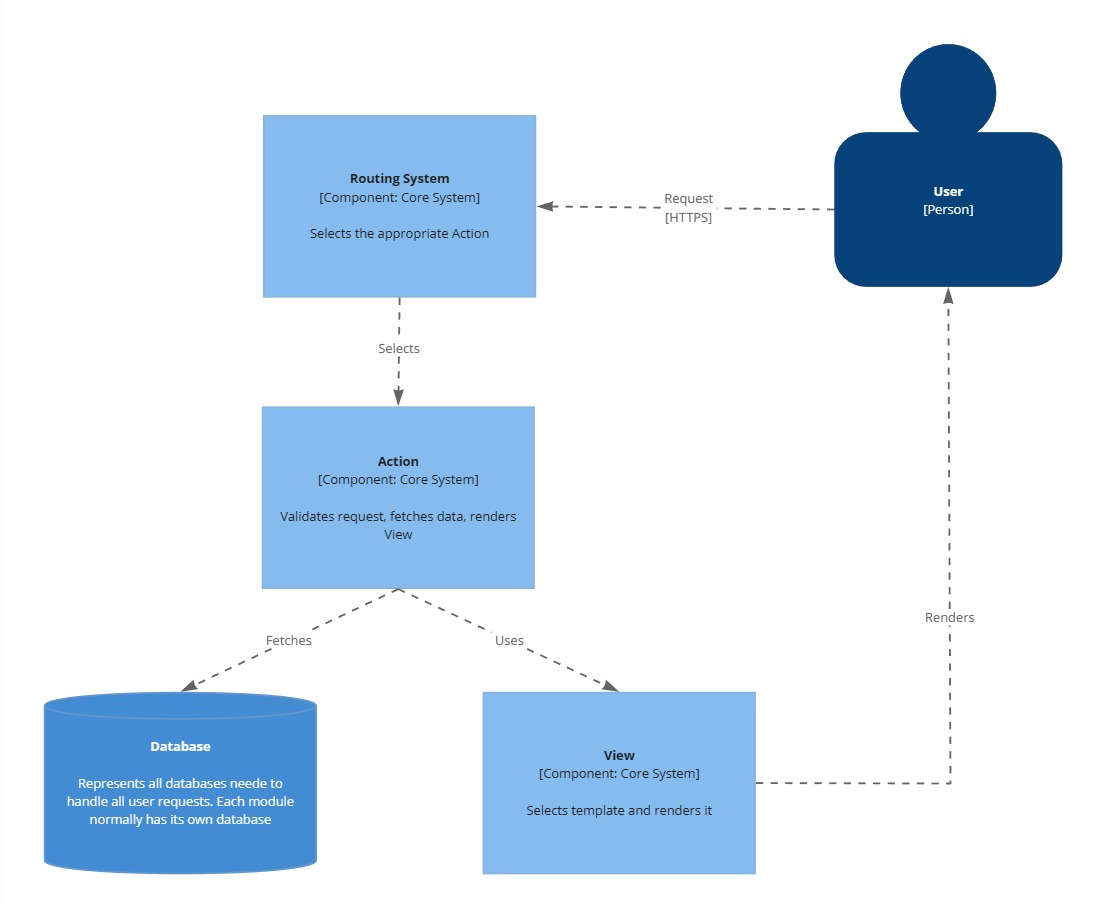
\includegraphics[width=0.75\linewidth]{images/c4-diagram}
    \caption{Architecture}
    \label{fig:architecture}
\end{figure}

The typical workflow consists of the following steps:

\begin{enumerate}
    \item Creation of request specific data objects and database connections are established.
    \item Execution of actions responsible for handling the request.
    \item Actions run business logic using database records or delegate processing to other system components.
    \item Response is aggregated and rendered in desired format to the user.
\end{enumerate}

\begin{figure}[H]
    \centering
    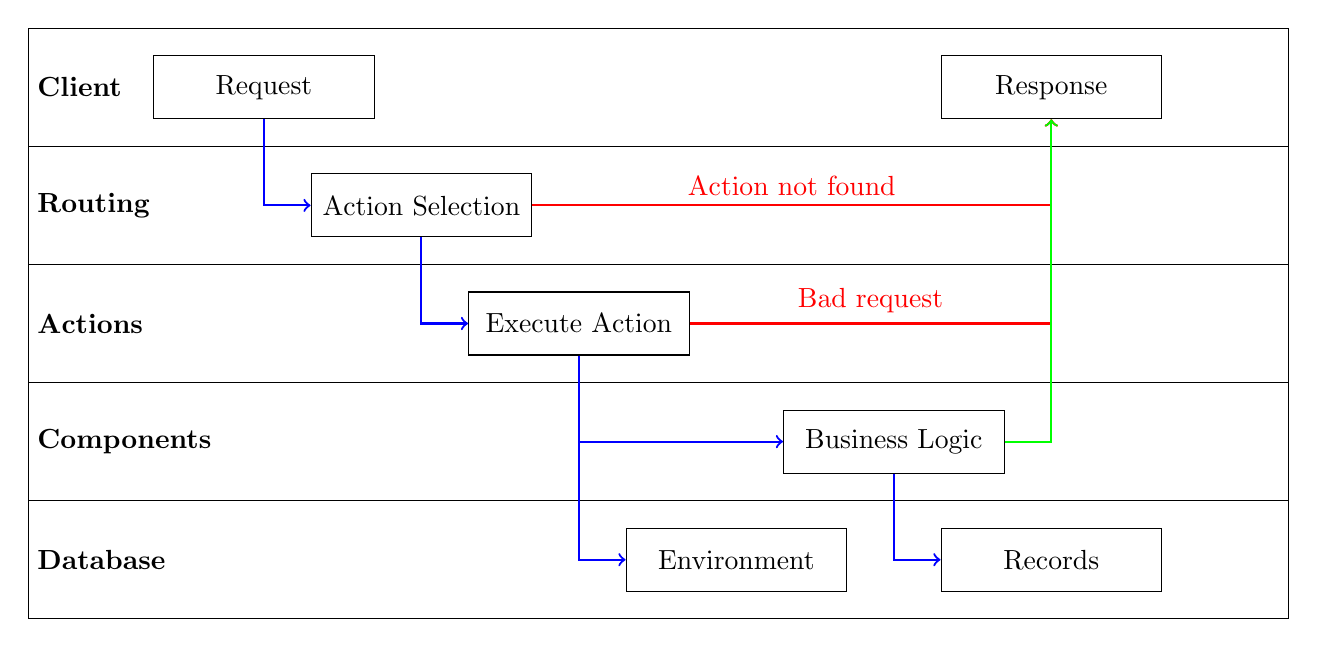
\begin{tikzpicture}
        [
        node distance=2.5cm,
        lane/.style={draw, minimum width=16cm, minimum height=1.5cm, anchor=west},
        activity/.style={draw, rectangle, minimum width=2.8cm, minimum height=0.8cm},
        arrow/.style={->, thick}
        ]

        \node[lane, label={[anchor=west]west:\textbf{Client}}] (client) at (0,4) {};
        \node[lane, label={[anchor=west]west:\textbf{Routing}}] (routing) at (0,2.5) {};
        \node[lane, label={[anchor=west]west:\textbf{Actions}}] (actions) at (0,1) {};
        \node[lane, label={[anchor=west]west:\textbf{Components}}] (components) at (0,-0.5) {};
        \node[lane, label={[anchor=west]west:\textbf{Database}}] (db) at (0,-2) {};

        \node[activity] (req) at (3,4) {Request};
        \node[activity] (response) at (13,4) {Response};

        \node[activity] (route) at (5,2.5) {Action Selection};

        \node[activity] (action) at (7,1) {Execute Action};

        \node[activity] (logic) at (11,-0.5) {Business Logic};

        \node[activity] (env) at (9,-2) {Environment};
        \node[activity] (query) at (13,-2) {Records};

        \draw[arrow, blue] (req) |- (route);
        \draw[arrow, blue] (route) |- (action);
        \draw[arrow, blue] (action) |- (logic);
        \draw[arrow, blue] (action) |- (env);
        \draw[arrow, blue] (logic) |- (query);

        \draw[arrow, red] (route) -| node[pos=0.25, above] {Action not found} (response);
        \draw[arrow, red] (action) -| node[pos=0.25, above] {Bad request} (response);

        \draw[arrow, green] (logic) -| (response);

    \end{tikzpicture}
    \caption{System Request Processing}
    \label{fig:system-request-processing}
\end{figure}

This pipeline-oriented design enables skipping defined steps if needed.

\subsection{Summary}\label{subsec:summary}
The proposed design emphasizes simplicity, abstraction, and extensibility.
Designing modern systems requires solving domain-specific problems while satisfying system constraints.
Simplicity and extensibility are two constraints that work against each other.
Simple solutions suffer from architectures that are difficult to extend, while extensible systems are overly reliant
on abstraction, leading to confusing APIs.
Implementing a complex design is an act of balancing between rigid architecture and convoluted abstractions.